\section{Propuesta}
\label{sec:propuesta-sol}
La propuesta para detectar fuga de información en aplicaciones Android, antes de
su publicación, consiste en proveer al desarrollador una herramienta para
análisis estático de flujos de información de la aplicación. Así, partiendo de
las anotaciones de seguridad que el desarrollador defina en el código fuente, se
verifica si la aplicación cumple con políticas de confidencialidad.\newline
Los requerimientos iniciales para construir tal herramienta son: un lenguaje
tipado de seguridad que permita anotar código fuente Android, y el conjunto de
reglas que evaluarán las políticas de confidencialidad.\newline 
Al consultar literatura científica al respecto, se encuentran herramientas como
JIF \ref{JIF-Tool} y JOANA \ref{JOANA-Tool}, especializadas en anotar código
Java, pero no código Android.
Si bien, ambas analizan flujos de información en aplicaciones Java, y podrían
ser extendidas para anotar código Android, las técnicas utilizadas por cada una
son diferentes, por un lado, JIF es un lenguaje tipado de seguridad que basa su
análisis en el chequeo de tipos. Por el otro, JOANA es un framework basado en
análisis de grafos de dependencia. Mientras JOANA se enfoca en precisión, JIF
posee un modelo de anotaciones (DLM) encargado de definir la lattice de
seguridad adecuada para las anotaciones en el código fuente, ofreciendo un
maduro sistema que además de evaluar políticas de confidencialidad, e
integridad, permite definir características de seguridad adicionales como
declasificación y endorsement.
Acorde a los propósitos del presente trabajo, JIF ofrece los beneficios de un
lenguaje tipado de seguridad y un sistema  sólido  de anotaciones, facilitando
la definición de las propiedades de seguridad a verificar.\newline 
Partiendo de JIF como el lenguaje tipado de seguridad, los retos subsiguientes
son: implementar el setup de JIF para Android e integrar a JIF un clasificador
para sources y sinks de Android. El setup de JIF para Android consiste en
implementar las adaptaciones necesarias para que el lenguaje JIF reconozca
código de la API de Android, y admita anotaciones JIF dentro de código
Android, pues aunque en esencia el código Android es código Java, JIF no tiene
como saberlo. También se requiere la integración de un clasificador de sources y
sinks al sistema de anotaciones de JIF, con el fin de proveer información
necesaria para evaluar las políticas de confidencialidad.\newline 
La figura \ref{fig:desing1-in} expone los elementos necesarios para construir la
herramienta de análisis. Básicamente, se requiere un módulo que extienda las
clases en JIF para que el lenguaje reconozca código de la API de Android, es
decir, para que admita anotaciones dentro del código Android: Setup extended JIF
classes. Un módulo que integre el clasificador de sources y sinks de Android al
sistema de anotaciones en JIF:  Android Sources and Sinks. Adicionalmente, se
requiere un modulo que evalúe las políticas de confidencialidad, Checking
Rule Sets, que debe tener comunicación con los módulos anteriormente descritos.
Como entrada, la herramienta recibe el código fuente de la aplicación,
debidamente anotado por el desarrollador, y parte de las anotaciones definidas
para retornar los resultados del análisis.\newline
Habiendo realizado las extensiones necesarias, se espera contar con una
herramienta de análisis de flujo de información, para un conjunto definido de
clases en Android. En la figura \ref{fig:desing1} se ilustra el comportamiento
esperado.\newline

\begin{figure}[t!]
	\begin{center}
	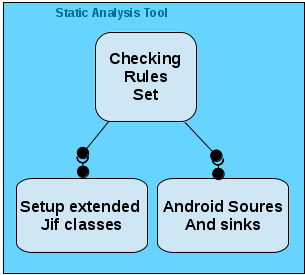
\includegraphics[width=4.6cm]{desing2-inside.png}
	\end{center}
	\caption{Static Analisys Tool Diagrama interno. Ilustra la composición interna
	de la herramienta propuesta para el análisis estático de aplicaciones Android.}
	\label{fig:desing1-in}
\end{figure}

\begin{figure}[t!]
	\begin{center}
	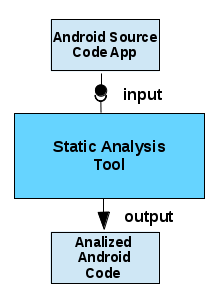
\includegraphics[width=3.5cm]{desing1-2.png}
	\end{center}
	\caption{Static Analisys Tool. Ilustra el input esperado por la herramienta, y
	el resultado devuelto.}
	\label{fig:desing1}
\end{figure} 

Luego, la estrategia de evaluación, consiste en verificar si la herramienta
implementada identifica pérdida de información mediante detección de flujos
implícitos. Esto debido a que, como se menciona en la descripción del problema,
parte importante de las propuestas para detección de fuga de información en
aplicaciones Android, hacen data-flow analysis aplicando técnicas de análisis
tainting, y en contraste con las técnicas de análisis de flujo de información,
las técnicas de análisis tainting no necesariamente consideran flujos
implícitos. Por tanto, al estar basada en JIF, cuyo enfoque de análisis es
precisamente flujo de información, se esperaría que la herramienta planteada
esté en capacidad de reconocer flujos implícitos.

% Se esperaría que: al realizar análisis de flujo de información aplicando
% técnicas Security-Typing, la herramienta propuesta, esté en capacidad de
% reconocer flujos implícitos.\newline
% Más específicamente, se puede tomar el conjunto de aplicaciones utilizadas como
% casos de prueba para la detección de flujos implícitos en
% DroidBench\cite{DroidBenchBenchmarks}, el benchmark de Flowdroid, y analizarlas
% con la herramienta propuesta.\newline

Más específicamente, se puede partir de DroidBench\cite{DroidBenchBenchmarks},
el benchmark de Flowdroid[\ref{FlowDroid-Tool}], tomar el conjunto de
aplicaciones con que prueban la detección de flujos implícitos, y analizarlas
con la herramienta propuesta.\newline
Finalmente estos resultados serían
comparados con los obtenidos mediante otras herramientas para análisis de fuga
de información en aplicaciones Android.\newline

En este orden de ideas, la evaluación de la herramienta propuesta está enfocada
en: medir recall frente a la detección de flujos implícitos, es decir, medir que
no genere falsos negativos ante la existencia de fugas de información,
provenientes de flujos implícitos.\newline

Por último, cabe anotar que aunque la presente propuesta está centrada en
verificar políticas de confidencialidad, en caso de contar con el tiempo
prudente, sería interesante analizar políticas adicionales como por ejemplo,
integridad y declasificación, pues estas son verificables mediante el modelo de
evaluación de JIF, modelo del que parte la herramienta de evaluación planteada.






